\subsection{Komplexe Zahlen}

Die Gleichung \(x^2=-1\) hat keine Lösung in \(\mathbb{R}\), da kein Quadrat einer
reellen Zahlen negativ sein.

Einführung der \enquote{imaginären Zahl} \(i = \sqrt{-1}\)

\[
	\mathbb{C} = \{z=a+ib \mid a,b \in \mathbb{R}\}
\]

Imaginäre Zahlen setzen sich aus einem Imaginärteil und einem Realteil zusammen
und werden in der \textit{Gaußschen Zahlenebene} (siehe Abb.~\ref{fig:gausche_zahlenebene}) dargestellt.

\begin{figure}
	\centering
	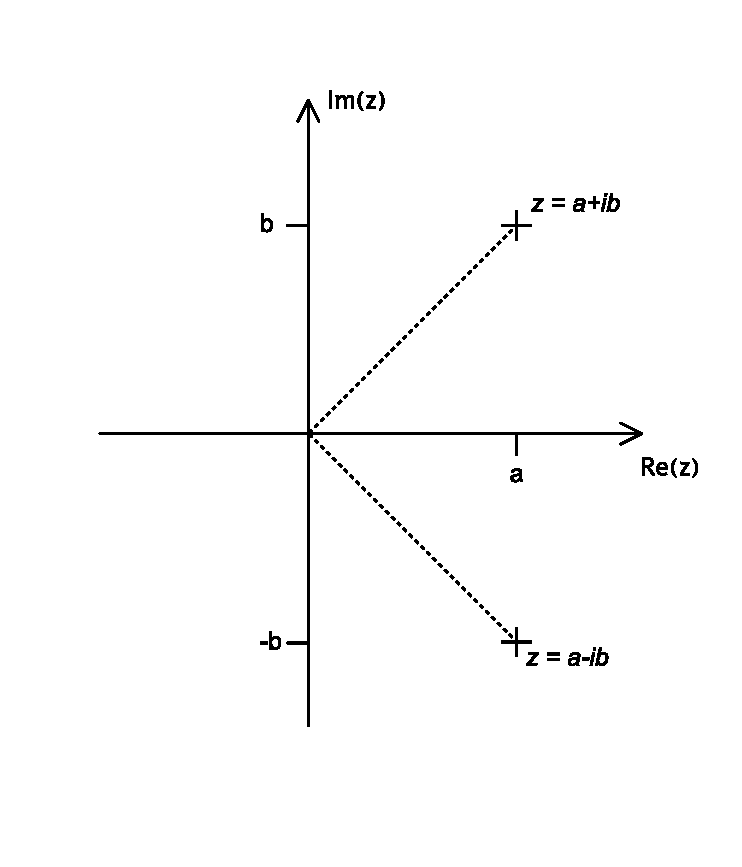
\includegraphics[scale=0.5]{grafiken/Komplexe_Zahlen}
	\caption{Die Gausche Zahlenebene}\label{fig:gausche_zahlenebene}
\end{figure}

\subsubsection{Algebraische Darstellungsform}


\begin{align*}
	z_1 & = a_1 + i b_1 \\
	z_2 & = a_2 + i b_2
\end{align*}


\subsubsection{Addition}


\begin{align*}
	z_3 & = z_1 + z_2                                       \\
	    & = (a_1 + i b_1) + (a_2 + i b_2)                   \\
	    & = a_1 + i b_1 + a_2 + i b_2                       \\
	    & = \underbrace{(a_1 + a_2)}_{a_3 \in \mathbb{R}} +
	\underbrace{i(b_1 + b_2)}_{b_3 \in \mathbb{C}}
\end{align*}

\subsubsection{Multiplikation}

\begin{align*}
	z_3 & = z_1 \cdot z_2                                         \\
	    & = (a_1 + i b_1) \cdot (a_2 + i b_2)                     \\
	    & = a_1 a_2 + a_1 ib_2 + ib_1 a_2 + ib_1 ib_2             \\
	    & = \underbrace{a_1 a_2 - b_1 b_2}_{a_3 \in \mathbb{R}} +
	\underbrace{i(a_1 b_2 + a_2 b_1)}_{b_3 \in \mathbb{C}}
\end{align*}


\subsubsection{Trigonometrische Darstellungsform}

\begin{figure}
	\centering
	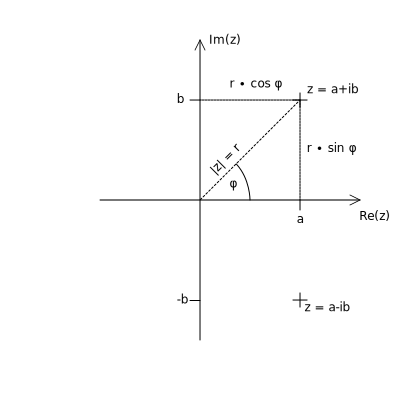
\includegraphics[scale=0.5]{grafiken/Komplexe_Zahlen_Herleitung}
	\caption{Die trigonometrische Darstellungsform von \(\mathbb{C}\)}\label{fig:trigonometrische_form}
\end{figure}

\[
	\begin{alignedat}{3}
		\vert z \vert &=\sqrt{a^2+b^2} \\
		\cos(\phi) &= \frac{a}{r} && \sin(\phi) &= \frac{b}{r} \\
		a &= r \cdot \cos(\phi) && r \cdot \sin(\phi) &= b \\
		z &= r \cos(\phi) + i r \sin(\phi) \\
		&= r (\cos(\phi) + i \sin(\phi))
	\end{alignedat}
\]

Vergleichend dazu siehe Abb.~\ref{fig:trigonometrische_form}.

\subsubsection{Eulersche Schreibweise}


\begin{align*}
	z & = r (\cos(\phi)) + i \cdot \sin(\phi) \\
	  & = r \cdot e^{i\ \phi}
\end{align*}

\subsubsection{Eulersche Gleichung}

\[
	\cos(\phi) + i \sin(\phi) = e^{i\ \phi}
\]

\paragraph{Multiplikation}

\begin{align*}
	z_1 & = r_1 \cdot e^{i\ \phi_1}                                                              \\
	z_2 & = r_2 \cdot e^{i\ \phi_2}                                                              \\
	\\
	z_3 & = z_1 \cdot z_2                                                                        \\
	    & = r_1 \cdot e^{i\ \phi_1} \cdot r_2 \cdot e^{i\ \phi_2}                                \\
	    & = \underbrace{r_1 r_2}_{r_3} \cdot \underbrace{e^{i(\phi_1 + \phi_2)}}_{e^{i\ \phi_3}}
\end{align*}

\begin{uebung}
	\begin{aufgabe}
		\[
			z^3 = 1
		\]
	\end{aufgabe}
	\begin{loesungsweg}
		\[
			\text{Es gilt:}
			r \cdot e^{i\ \phi} = z
		\]

		\subparagraph{Berechnung von \(z_1\):}


		\begin{align*}
			z^3 & = {\left(r \cdot e^{i\ \phi}\right)}^3                                           \\
			z^3 & = r^3 \cdot e^{3 i\ \phi}                                                        \\
			1   & = r^3 \cdot e^{3 i\ \phi}                                                        \\
			1   & = r(\underbrace{\cos{(3 \phi)}}_{=1} + \underbrace{i \cdot \sin{(3 \phi)}}_{=0})
		\end{align*}

		\subparagraph{Berechnung von \(z_2\) und \(z_3\):}

		\[
			\begin{alignedat}{1}
				\cos{(3 \phi)} &= 1 \\
				3 \phi &= 2 \pi \\
				\phi &= \frac{2}{3} \pi \\
				\text{Es gilt aber auch:} \\
				3 \phi &= 4 \phi \\
				\phi &= \frac{4}{3} \pi
			\end{alignedat}
		\]
	\end{loesungsweg}

	\begin{loesung}
		\[
			\begin{alignedat}{3}
				z_1    &     & z_2       &                   & z_3       &                   \\
				r_1    & = 1 & \quad r_2 & = 1               & \quad r_3 & = 1               \\
				\phi_1 & = 0 & \phi_2    & = \frac{2}{3} \pi & \phi_3    & = \frac{4}{3} \pi
			\end{alignedat}
		\]
	\end{loesung}
\end{uebung}
